%%%%%%%%%%%%%%%%%%%%%%%%%%%%%%%% Introducción:
\begin{frame}[fragile]{Alternativas.}{}
  \begin{wrapfigure}{r}{0.25\textwidth} %this figure will be at the right
    \centering
    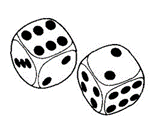
\includegraphics[width=0.25\textwidth]{./Imagenes/Aleatorios.png}
    \caption*{Aleatorios.}
  \end{wrapfigure}
  
  Algunas alternativas para agrupar son:
  \begin{enumerate}
  \item \textbf{Redes neuronales}.
  \item \textbf{k-means $+$ Algoritmos genéticos}.
  \item \textbf{Muestreos aleatorios}.
  \end{enumerate}

%  \begin{wrapfigure}{l}{0.25\textwidth}
%    \centering
%    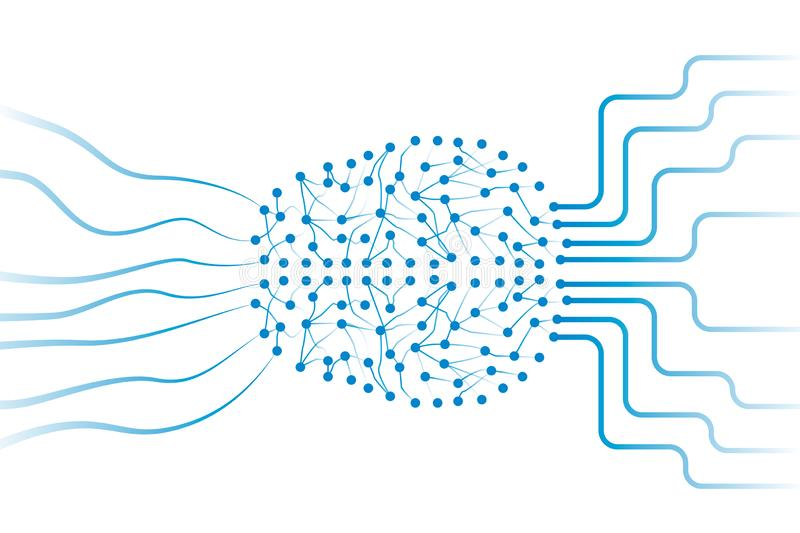
\includegraphics[width=0.25\textwidth]{Imagenes/RedNeuronal.jpg}
%  \end{wrapfigure}
  \begin{justify}  
    Algunas alternativas para agrupar basadas en el entrenamiento inteligente,
    búsquedas aleatorias (como las heurísticas), y uso de algoritmos genéticos
    (como las colonias de hormigas) son recurridas cuando no podemos garantizar
    un ``buen'' agrupamiento.
  \end{justify}
  
  \begin{figure}
    \centering
    \begin{subfigure}[b]{0.3\textwidth}
      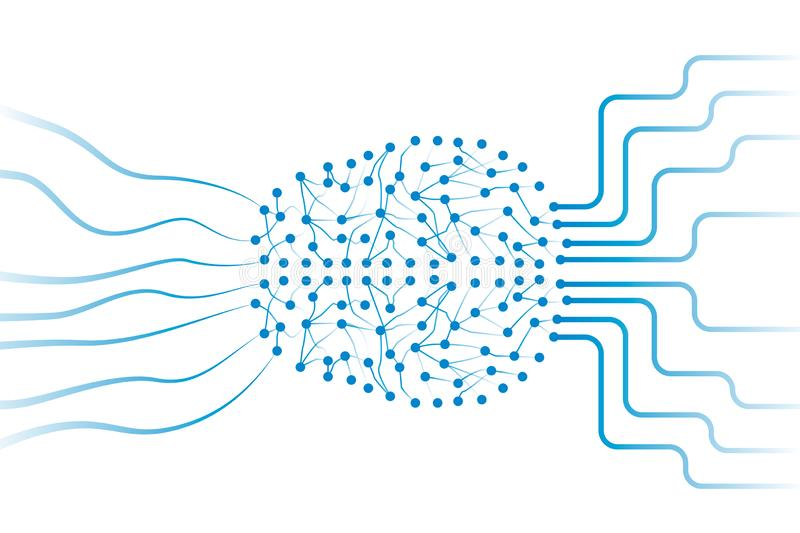
\includegraphics[width=\textwidth]{./Imagenes/RedNeuronal.jpg}
      \caption*{Redes Neuronales.}
    \end{subfigure}
    \begin{subfigure}[b]{0.3\textwidth}
      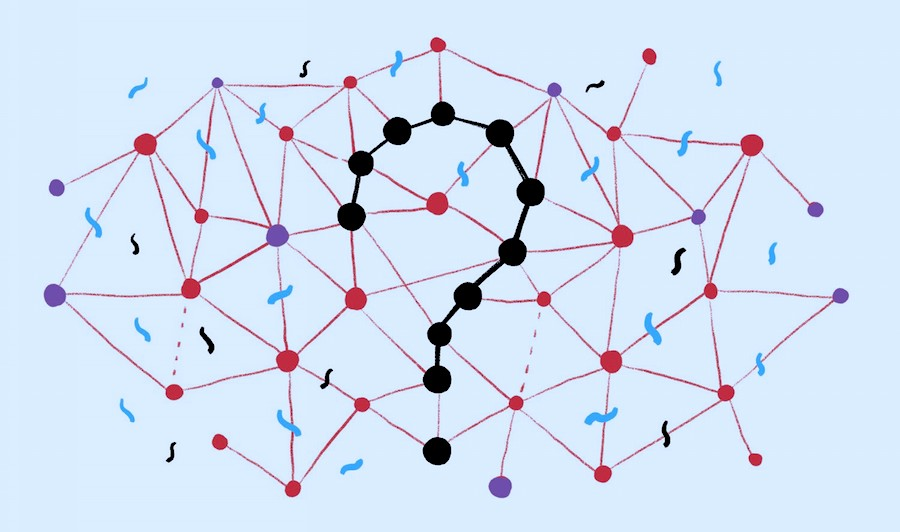
\includegraphics[width=\textwidth]{./Imagenes/Geneticos.jpeg}
      \caption*{K-means + Genéticos.}
    \end{subfigure}
  \end{figure}
\end{frame}
